% kate: word-wrap true;

\chapter{Writing system}
\index{Tahano Hikamu|(}

In the previous chapter, example words were given in Ayeri's script, \rayr{thno 
hikmu}{Tahano Hikamu}, wherever possible. Thus, it seems advisable to include a 
description of Ayeri's native writing system here as well. Literally, 
\rayr{thno hikmu}{Tahano Hikamu} means `Round Script' (script round), which is 
an old formation based on the word \xayr{thnF/}{tahan-}{write} that  stuck. The 
current word for `script' is \xayr{thnnF}{tahanan}{writing}. Tahano Hikamu was 
originally named thus because of an earlier draft for a script that never made 
it very far beyond the drawing board and which was a lot more angular and boxy, 
see \autoref{fig:boxyhikamu}---Tahano Hikamu was a lot more bubbly in 
comparison, especially early on (\autoref{fig:th2005}).\footnote{Unfortunately, 
there is no documentation of the Box script surviving that I know 
of.}\index{Box script}

\begin{figure}[tp]
\caption{Box script and Hikamu}

\begin{minipage}{.5\linewidth}
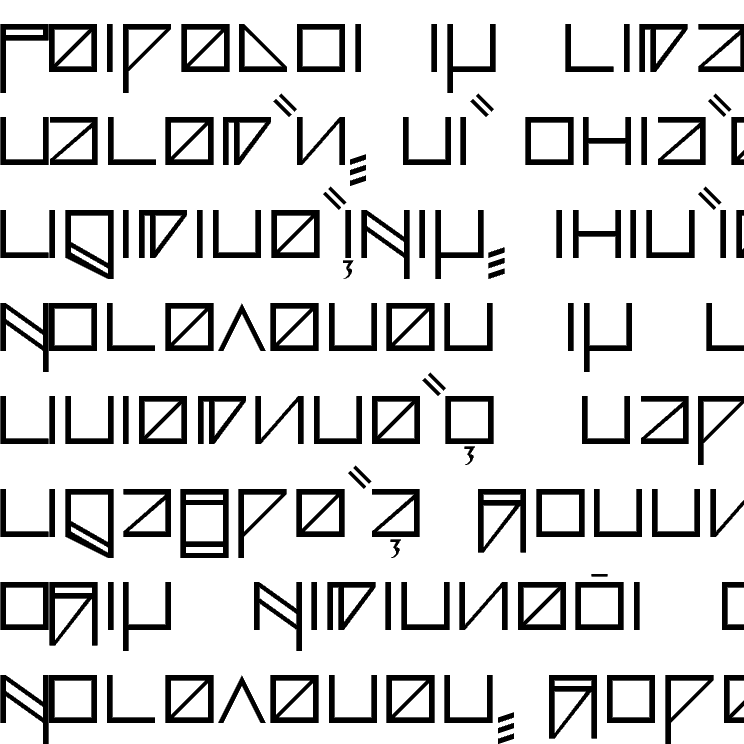
\includegraphics[width=\linewidth]{images/hinya-300dpi-clip.png}
\subcaption{Old and aborted draft: Box script}
\label{fig:boxy}
\end{minipage}
~
\begin{minipage}{.5\linewidth}
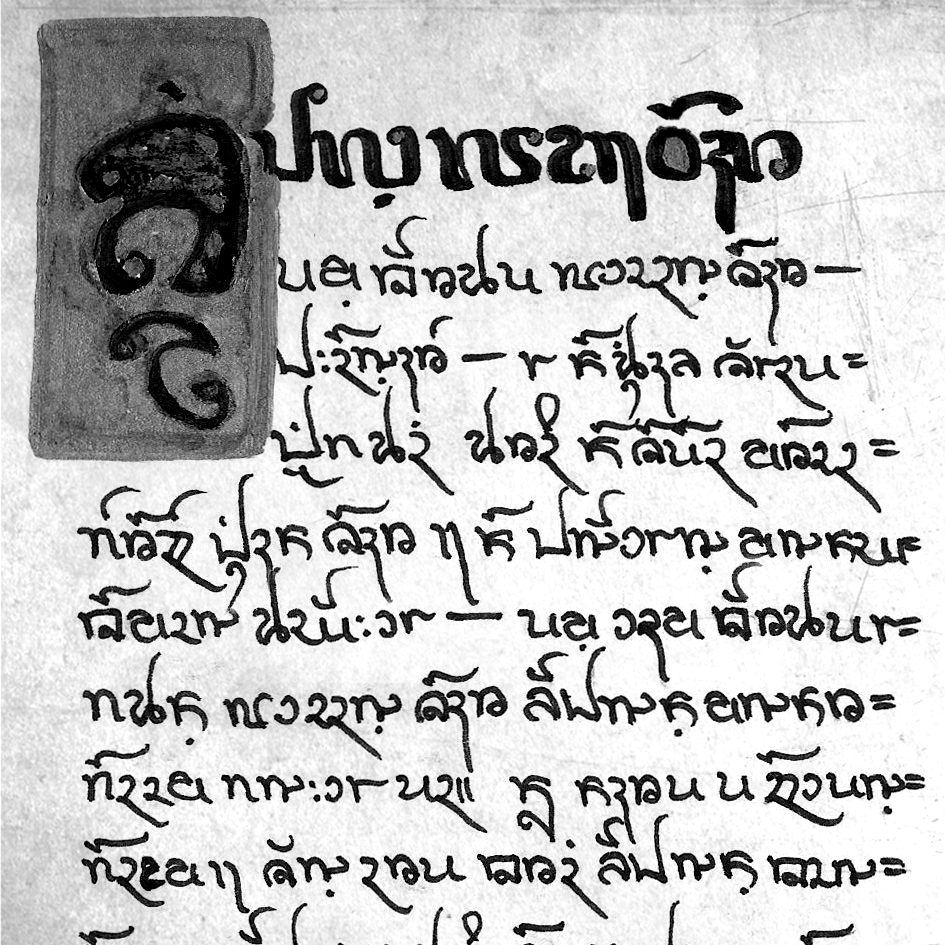
\includegraphics[width=\linewidth]{images/tahano-300dpi-bw-clip.png}
\subcaption{Ayeri's native script: Tahano Hikamu}
\end{minipage}

\label{fig:boxyhikamu}
\end{figure}

As we have seen in the previous chapter, Ayeri's prosody strongly emphasizes 
the syllable as a unit. Thus, it is not a surprise that Ayeri's native script,
Tahano Hikamu, is an alphasyllabary similar to the Brāhmī alphabets of 
India and Southeast Asia \parencites{salomon1996}{court1996}.\index{Brāhmī 
scripts} Scripts like these are 

\blockcquote[376]{salomon1996}{based on the unit of the graphic 
\enquote{syllalbe} […], which by definition always ends with a vowel (type V, 
CV, CCV, etc.). Syllables consisting of a vowel only (usually at the beginning 
of a word or sentence) are written with the \emph{full} or \emph{initial vowel 
signs} […]. But when, as is much more frequently the case, the syllable 
consists of a consonant followed by a vowel, the vowel is indicated by a 
diacritic sign attached to the basic sign for the consonant […].}

For Tahano Hikamu the definition that a syllable consisting only of a vowel is 
written with an initial vowel sign is only true under certain circumstances, as 
we will see below. Moreover, Brāhmī scripts are often characterized by 
conjuncts of clustered consonants which may become quite large and sometimes 
behave in an idiosyncratic way. Consonant conjuncts like Devanāgarī {\FS 
त्व}~\orth{tva} from {\FS त}~\orth{ta} + {\FS व}~\orth{va} or idiosyncratic 
conjuncts like {\FS क्ष} \orth{kṣa} for {\FS क} \orth{ka} + {\FS ष} \orth{ṣa} 
are not known in Tahano Hikamu, however. Tahano Hikamu also does not know 
subscript notation for consonant clusters and special diacritics marking coda 
consonants like in Javanese \citep[478--479]{kuipersmcdermott1996}. This does 
not mean, however, that final consonants are simply omitted in writing, since 
closed syllalbes are reasonably common enough in Ayeri to warrant indicating 
them. Thus, there is \textcquote[476]{kuipersmcdermott1996}{a special mark to 
eliminate the vowel of the previous syllable, thereby leaving a consonant in a 
syllable-final position.} That is, a diacritic exists which marks the absence 
of an inherent vowel, rendering the syllable consonant-only.

Another difference from Brāhmī-family scripts is that vowel length and 
diphthongs in [ɪ] are indicated by dedicated diacritics, so the long vowels 
are not doubled versions of their short counterparts. Like in 
Kharoṣṭhī---another historically important ancient script of India---initial 
vowels are not represented by unique graphemes but they are all written like 
post-consonantal vowel diacritics \citep[377]{salomon1996}, though in Tahano 
Hikamu with a charcter without an inherent sound value. For this reason, 
the character is indicated in the table below as \ayr{ʔ} /Ø/; its native name 
is \xayr{rnYn}{ranyan}{nothing}.\footnote{I will give the native names of 
graphemes here, but will refer to them by their English names for clarity in 
the running text.} Similar to a number of Brāhmī scripts, Tahano Hikamu puts 
diacritics not only below or above consonant bases, but also before them. This, 
however, is not limited to vowel graphemes as in Devanāgarī {\FS ि}~\orth{i} or 
Javanese \smash{\fontspec{Tuladha Jejeg}[Script=Javanese, 
Scale=MatchLowercase]ꦺ}~\orth{e, é/è} 
\citep[478]{kuipersmcdermott1996}.\footnote{\citet{kuipersmcdermott1996} do not 
say, but it looks likely to me that both are related, since they are both 
functionally the only prepended vowel diacritics and both represent a high front 
sound.}

\section{Consonants}
\index{consonants|(}

Tahano Hikamu is mainly based on consonant bases that are modified by 
diacritics. Since the vowel /a/ is so highly frequent in Ayeri, it is also the 
vowel that is \fw{inherent} to every consonant grapheme if not further modified 
by vowel diacritics. Consonant letters are simply referred to as \textit{pa, ta, 
ka, ...} \autoref{fig:consonants} displays all the main consonants. The 
customary collation is---similar to the IPA table---roughly grouping the letters 
according to their sound value by anteriority (front → back) and sonority (low → 
high). The script is monocameral, that is, there is no distinction between 
capital letters and minuscule letters as in the Latin, Greek, Cyrillic, 
Georgian, and Armenian alphabet. It is also written in lines from left to right.

% \begin{center}\itshape
% 	pa, ta, ka;\\
% 	ba, da, ga;\\
% 	ma, na, nga;\\
% 	va, sa, ha;\\
% 	ra, la, ya;\\
% 	Ø.\\
% \end{center}

\begin{figure}[ht]
\caption{The consonant graphemes}

\begin{tabu} to \linewidth{X[c] X[c] X[c] X[c] X[c] X[c]}
\toprule
\tableheaderfont	/pa/ & /ta/ & /ka/ & /ba/ & /da/ & /ga/ \\
\rowfont{\Tagati\huge}	p & t & k & b & d & g \\

\midrule

\tableheaderfont	/ma/ & /na/ & /ŋa/ & /va/ & /sa/ & /ha/ \\
\rowfont{\Tagati\huge}	m & n & N & v & s & h \\

\midrule

\tableheaderfont	/ra/ & /la/ & /ja/ & /Ø/ \\
\rowfont{\Tagati\huge}	r & l & y & ʔ \\

\bottomrule
\end{tabu}
\label{fig:thcons}
\end{figure}

\ayr{ʔ}, which in Ayeri has no sound value but is used as a base for initial 
vowels, may also serve as the character for /ʔa/. What is, moreover, 
interesting about \ayr{N}~\orth{nga} is that even though before, /ŋ/ was 
treated 
strictly as a coda consonant in the previous chapter, it is in fact treated as 
an onset consonant in writing if a vowel is following:

\ex[lingstyle=thex]\begingl
	\gla \ayr{p}	$+$	\ayr{NisF} //
	\glb /pa/	{}	/ŋis/ //
	\glft \rayr{\larger pNisF}{pangis} /paŋ.is/ `money' //
\endgl\xe

Tahano Hikamu knows a few ligatures. First of all, when two \ayr{n} \orth{na} 
are in succession within a word, they will form a ligature \ayr{nn} \orth{nana}:

\ex[lingstyle=thex]\begingl
	\gla \ayr{n}	$+$	\ayr{n}	→	\ayr{nn} //
	\glb /na/	{}	/na/	{}	/nana/ //
\endgl\xe

\noindent This is distinct from conjuncts like in Devanāgarī et al., though, 
since the unmodified sound value will still be /nana/, not */nna/, so the 
inherent vowel of each \ayr{n} \orth{na} is not deleted, and each \ayr{n} 
\orth{na} retains the ability to be modified by diacritics. Tahano Hikamu also 
has a few ligatures of the kind you would find in Brāhmī scripts, however:

\pex
	\a \ayr{\larger q}~\orth{kwa} ← \ayr{\larger k}~\orth{ka} + 
		\ayr{\larger v}~\orth{va},
	\a \ayr{\larger T}~\orth{tsa} ← \ayr{\larger t}~\orth{ta} + 
		\ayr{\larger s}~\orth{sa}, and 
	\a \ayr{\larger x}~\orth{ksa} ← \ayr{\larger k}~\orth{ka} + 
		\ayr{\larger s}~\orth{sa}.
\xe

\noindent These conjunct letters are, however, not normally employed by Ayeri. 
\autoref{fig:thconsadd} shows all additional consonants, added to write other 
languages. Individual languages may adapt the sound values slightly to fit 
their 
own purposes.

\begin{figure}[ht]
\caption{Additional consonant graphemes}

\begin{tabu} to \linewidth{X[c] X[c] X[c] X[c] X[c] X[c]}
\toprule
\tableheaderfont	/fa/ & /wa/ & /tsa/ & /za/ & /ʃa/ & /ʒa/ \\
\rowfont{\Tagati\huge}	f & w & T & z & S & Z \\

\midrule

\tableheaderfont	/ça/ & /ksa/ & /kwa/ & /xa/ & /ɣa/ \\
\rowfont{\Tagati\huge}	C & x & q & X & G \\

\bottomrule
\end{tabu}
\label{fig:thconsadd}
\end{figure}

\index{consonants|)}

\section{Vowels}
\index{vowels|(}

As mentioned above, vowels are written as diacritics that are added to 
consonants. In principle, every consonant has two slots for vowels, a primary 
one atop it, and a secondary one below it. Vowels added to consonants in 
the primary slot delete their inherent /a/:

\ex[lingstyle=thex]\begingl
	\gla \ayr{p}	→	\ayr{pe} //
	\glb /pa/	{}	/pe/ //
\endgl\xe

\begin{figure}[th]
\caption{Primary vowel graphemes}

\begin{tabu} to \linewidth{H[c] X[c] X[c] X[c] X[c] X[c] X[c] X[c]}
\toprule
\tableheaderfont

	& /i/
	& /e/
	& /a/
	& /o/
	& /u/
	& /ə/
	& /aʊ/
	\\
	
\toprule
	
Diaritics
	& \Tagati\huge *i
	& \Tagati\huge *e
	& \huge ({\Tagati *a})
	& \Tagati\huge *o
	& \Tagati\huge *u
	& \Tagati\huge *ə
	& \Tagati\huge *au
	\\

\midrule

Independent
	& \Tagati\huge I
	& \Tagati\huge E
	& \Tagati\huge A
	& \Tagati\huge O
	& \Tagati\huge U
	& \Tagati\huge Ə
	& \Tagati\huge AU
	\\

\bottomrule
\end{tabu}
\label{fig:thvowstop}
\end{figure}

\autoref{fig:thvowstop} gives the primary vowel signs. Of the vowel signs given 
there, only \ayr{*ə}~\orth{ə} is not used in Ayeri. \ayr{*au}~\orth{au} is the 
only diphthong for which a dedicated grapheme exists, even though its 
occurrence 
is rather limited. The independent vowel graphemes are used at the beginning of 
words or inside words when there is no other way to spell the vowel, which is 
occasionally the case for secondary vowels. Secondary vowels are vowels that 
are 
not parts of diphthongs (even though another language might use them to spell 
diphthongs that are not covered by default), but follow the vowel of a syllable 
directly. They are attached underneath a consonant base, for example:

\ex[lingstyle=thex]\begingl
	\gla \ayr{y}	→	\ayr{ye}	→	\ayr{ye\_a} //
	\glb /ja/	{}	/je/		{}	/jea/ //
\endgl\xe

In fact, the principle that every consonant base with its diacritics represents 
one syllable is slightly violated here, which is also the reason why secondary 
vowels very occasionally need to be spelled as independent vowels, for example 
when the secondary vowel is long, as in the word \xayr{ruAAnF}{ruān}{duty}:

\ex[lingstyle=thex]\label{ex:rwaa}\begingl
	\gla \ayr{ru}	→	\ayr{ruAA}	\quad	(\,\ayr{ruu\_a}) //
	\glb /ru/	{}	/rwaː/ 		\quad	/ruːa/ //
\endgl\xe

Example (\ref{ex:rwaa}) uses a diacritic, \ayr{*aa}, to indicate length. If 
is put directly under \rayr{ru}{ru} (the \ayr{*\_a} diacritic moves down where 
it is not in the way), the syllable will incorrectly spell /ruːa/ instead of 
the intended /ruaː/. This is because diacritics modify consonants and primary 
vowels, but there is no way to modify a secondary vowel directly. 
\autoref{fig:thvowsbot} gives a list of secondary vowels corresponding to that 
of primary vowels above. The vowels as well are just referred to by their sound 
value; `primary' and `secondary', `superscript' and `subscript' or `upper' and 
`lower' may be chosen to disambiguate their positions; the native names may use 
\xayr{Iraj}{iray}{high} and \xayr{Ejr}{eyra}{low} to disambiguate, so \rayr{E 
Irj}{e iray} denotes the superscript \orth{e} diacritic while \rayr{E Ejr}{e 
eyra} denotes its subscript counterpart.

\begin{figure}[ht]
\caption{Secondary vowel graphemes}

\begin{tabu} to \linewidth{X[c] X[c] X[c] X[c] X[c] X[c] X[c]}
\toprule
\tableheaderfont	/i/ & /e/ & /a/ & /o/ & /u/ & /ə/ & /aʊ/ \\
\rowfont{\Tagati\huge}	*\_i & *\_e & *\_a & *\_o & *\_u & *\_ə & *\_au \\

\bottomrule
\end{tabu}
\label{fig:thvowsbot}
\end{figure}

As a further exception, those consonant bases with an ascender 
(\ayr{k}~\orth{ka}, \ayr{d}~\orth{da}, \ayr{C}~/ça/) move the primary vowel to 
the secondary slot below the consonant by default while indicating the vacancy 
of the primary slot at the top with a dot. This is done to avoid crossing the 
ascender of the consonant with a vowel diacritic:

\ex[lingstyle=thex]\begingl
	\gla \ayr{k}	→	\ayr{k\_i}	→	\ayr{ki} //
	\glb /ka/	{}	/ka.i/		{}	/ki/ //
\endgl\xe

If the primary vowel slot were not silenced by the \ayr{*\_F} diacritic, it 
could reasonably be assumed that the consonant is not losing its inherent /a/ 
and the vowel below the consonant indicates a secondary vowel, spelling /CaV/. 
If, however, a secondary vowel is \emph{actually} added, primary and secondary 
vowels will be assigned the regular primary and secondary slots, respectively, 
again (\ref{ex:kie}). This condition also holds true for subscript diacritics 
(\ref{ex:kii}).

\pex[lingstyle=thex]
\a\label{ex:kie}\begingl
	\gla \ayr{ki}	→	\ayr{ki\_e} //
	\glb /ki/	{}	/ki.e/ //
\endgl

\a\label{ex:kii}\begingl
	\gla \ayr{ki}	→	\ayr{kii} //
	\glb /ki/	{}	/kiː/ //
\endgl

\xe

The order of secondary vowels and subscript diacritics is iconic insofar as 
it follows the order of sounds in the syllable. Thus, secondary vowels appear 
below the consonant-doubling diacritic, \ayr{*F*}, while they appear above the 
syllable-final homorganic nasal diacritic, \ayr{*\_M}:

\pex[lingstyle=thex]\label{ex:subscrord}
\a\begingl
	\gla \ayr{pFp}	→	\ayr{pFpe\_a} //
	\glb /ppa/	→	/ppea/ //
\endgl

\a\begingl
	\gla \ayr{peM}	→	\ayr{pe\_aM} //
	\glb /peN/	→	/peaN/ //
\endgl
\xe

\index{vowels|)}

\section{Diacritics}
\index{diacritics|(}

We have already encountered a few diacritics, though Tahano Hikamu comes with 
a lot more, some of which undergo non-trivial positioning and repositioning 
rules. As vowels are primarily expressed as superscripts, diacritics are 
primarily realized as subscripts, so in the following I will first describe 
subscript diacritics; then prepended diacritics, which Ayeri also has a number 
of, both as graphemes in their own right and as allographs of other subscript 
diacritics; and then, lastly, superscript diacritics.

\subsection{Subscript diacritics}

\begin{sidewaysfigure}[p]
\caption{Bottom-attaching diacritics}
\begin{tabu} to \linewidth{>{\Tagati\huge}X[1] X[8l] X[16l] X[12l]}
\toprule
\tableheaderfont

	& Native name
	& Function
	& Example
	\\
	
\toprule

\tablesubheaderfont\multicolumn{4}{c}{L~a~r~g~e~{ }~d~i~a~c~r~i~t~i~c~s}\\

\midrule

*aa
	& \xayr{tupsti}{tupasati}{long-maker}
	& Lengthens the primary vowel of the syllable
	& \rayr{p}{pa} → \rayr{paa}{pā}
	\\

\midrule
	
*Y
	& \xayr{y Ejr}{ya eyra}{low ya}
	& \orth{ya} following another consonant, also across syllables. Marks 
		palatalization of \ayr{t}~\orth{ta}, \ayr{d}~\orth{da}, 
		\ayr{k}~\orth{ka}, \ayr{g}~\orth{ga} and \ayr{y}~\orth{ya} in 
		Ayeri.
	& \rayr{Ar}{ara} → \rayr{ArY}{arya}; \rayr{t}{ta} → \rayr{tY}{ca}
	\\
	
\midrule
	
*J
	& \xayr{riNy}{ringaya}{raiser}
	& Palatalizes a consonant (not used in Ayeri)
	& \rayr{t}{ta} → \ayr{tJ} /tʲa/, /tʃa/
	\\
	
\midrule
	
*H
	& \xayr{UlNy}{ulangaya}{breather}
	& Aspiration or frication of a consonant (not used in Ayeri)
	& \rayr{t}{ta} → \ayr{tH} /tʰa/, {\addfontfeature{RawFeature=+mgrk}/θa/}
	\\
	
\midrule
	
*\hspace{-.25em}ˀ
	& \xayr{rjpaay Ejr}{raypāya eyra}{low~stopper}
	& Glottal stop coda or glottalization of a consonant (consonant letters 
		with ascenders; not used in Ayeri)
	& \rayr{k}{ka} → \ayr{kQ} /kaʔ/; \rayr{d}{da} → \ayr{dQ} /d’a/
	\\

\midrule

\tablesubheaderfont\multicolumn4{c}{S~m~a~l~l~{ }~d~i~a~c~r~i~t~i~c~s}\\

\midrule

*F
	& \xayr{goMdy}{gondaya}{extinguisher}
	& Deletes the inherent /a/ of a consonant, e.g. in consonant clusters 
		or closed syllables
	& \rayr{pr}{para} → \rayr{pFr}{pra}, \rayr{prF}{par}
	\\
	
\midrule
	
*M
	& \xayr{vinaati}{vināti}{nasalizer}
	& Indicates a homorganic nasal or nasalizes the vowel, depending on the 
		language
	& \rayr{pd}{pada} → \rayr{pMd}{panda} /panda/ or /pãda/
	\\
	
\midrule
	
*F*
	& \xayr{kusNisaati}{kusangisāti}{duplicator}
	& Indicates a geminated or otherwise double consonant
	& \rayr{pl}{pala} → \rayr{plFl}{palla}
	\\

\bottomrule
\end{tabu}
\label{fig:thdiabot}
\end{sidewaysfigure}

\autoref{fig:thdiabot} shows the bottom-attaching diacritics. The `large 
diacritics' cause the secondary slot of consonants to move down below the 
diacritic. `Small diacritics' can attach in this place as well as secondary 
vowels, as does the homorganic nasal diacritic \ayr{*M} in this 
diacritic-fraught example:

\ex[lingstyle=thex]\label{ex:caampuluy}\begingl
	\gla \ayr{tYaan} $+$ \ayr{puluj} → \ayr{tYaaMpuluj} //
	\glb {/ˈtʃaːn/} {} {/puˈlʊɪ/} {} {/ˌtʃaːmpuˈlʊɪ/} //
% 	\glc \xayr{tYaanF}{cān}{love} {} \xayr{puluj}{puluy}{opposite} {}
% 		\xayr{tYaaMpuluj}{cāmpuluy}{heterosexual} //
	\glft \xayr{\larger tYaaMpuluj}{cāmpuluy}{heterosexual} //
\endgl\xe

It also needs to be noted that diacritics like \ayr{*Y} are applied 
progressively to words as a whole, not stopping at morpheme and syllable 
boundaries, so even though \tayr{toryeng}{she sleeps} may be composed of 
\xayr{torF/}{tor-}{sleep} + \rayr{/yeNF}{-yeng} (=\TsgF{}.\Aarg{}) and 
syllabifies as /tor.ˈjeŋ/, the spelling is not *\,\ayr{torF\zwsp{}yeNF} as one 
might expect, but \ayr{torYeNF}.

Even though the primary position for small diacritics is underneath consonants, 
the diacritic deleting the inherent vowel, \ayr{*F}, very commonly also 
appears after a consonant letter at the end of words:

\ex[everygla=\Tagati\Large,everyglb=\itshape]\begingl
	\gla y nimFreN\thafterdot{} pNn\thafterdot{} 
		nraanFyen. //
	\glb Ya nimreng pangan narānyena. //
	\glc Ya nim-reng pangan-Ø narān-ye-na //
	\glc \LocT{} appear=\TsgI{}.\Aarg{} end-\Top{} word-\Pl{}-\Gen{} //
	\glft `It appears at the end of words.' //
\endgl\xe

This strategy is advantageous in that Tahano Hikamu leaves very little space 
between individual words: \ayr{y nimFreN\thafterdot{} pNn\thafterdot{} 
nraanFyen.} With the dot after the consonant, word boundaries are more visible.

\subsection{Prepended diacritics}

Example (\ref{ex:caampuluy}) leads us directly to the next class of 
diacritics---ones that are prepended to the consonant letter, either because 
they are simply placed there or because of allography. Let us first list those 
diacritics that appear in front of consonants obligatorily 
(\autoref{fig:thdiapreobl}).

\begin{figure}[htp]
\caption{Obligatorily prepended diacritics}
\begin{tabu} to \linewidth{>{\Tagati\huge}X[1] X[8l] X[16l] X[12l]}
\toprule
\tableheaderfont

	& Native name
	& Function
	& Example
	\\
	
\toprule

*j
	& \xayr{leMtMkusNF}{lentan\-kusang}{double-\allowbreak{}sound}
	& Marks a diphthong with /ɪ/
	& \rayr{pe}{pe} → \rayr{pej}{pey}
	\\
	
\midrule

*\_:
	& \xayr{tilmy}{tilamaya}{changer}
	& Marks raised vowels (i.e. umlaut; not used in Ayeri)
	& \rayr{po}{po} → \ayr{po\_:}~/pø/
	\\
	
\midrule

*R
	& \xayr{hiymy}{hiyamaya}{roller}
	& Marks retroflex consonants (not used in Ayeri)\footnotemark
	& \rayr{t}{ta} → \ayr{tR}~/ʈa/
	\\

\bottomrule
\end{tabu}
\label{fig:thdiapreobl}
\end{figure}

\footnotetext{In a Tahano Hikamu orthography I devised for English once, 
\ayr{*R} was used for /ɚ/, as in the \textsc{nurse} vowel in American English: 
\rayr{nRsF}{nurse}.}

\begin{figure}[htp]
\caption{Allographically prepended diacritics}
\begin{tabu} to \linewidth{>{\Tagati\huge}X[1] X[8l] X[16l] X[12l]}
\toprule
\tableheaderfont

	& Native name
	& Function
	& Example
	\\
	
\toprule

ː*
	& \xayr{tupsti mrinF}{tupasati marin}{anterior long-maker}
	& Lengthens the primary vowel of the syllable
	& \rayr{sY}{sya} → \rayr{sYaa}{syā},\newline
		\rayr{n}{na} → \rayr{naa}{nā}
	\\
	
\midrule

ʲ*
	& \xayr{y mrinF}{ya marin}{anterior ya}
	& \orth{ya} following another consonant, also across syllables.
	& \rayr{n}{na} → \rayr{nY}{nya}
	\\
	
	
	& \xayr{riNy mrinF}{ringaya marin}{anterior raiser}
	& Also used as an allograph for the palatalization proper diacritic.
	& \ayr{sH}~/sʰa/ → \ayr{sHY}~/sʰʲ/
	\\
	
\midrule

ʰ*
	& \xayr{UlNy mrinF}{ulangaya marin}{anterior breather}
	& (Pre-)Aspiration or frication of a consonant (not used in Ayeri)
	& \rayr{N}{nga} → \ayr{NH} /ŋʰa/;\newline
		\rayr{t}{ta} → \ayr{ʰt}~/ʰta/
	\\

\bottomrule
\end{tabu}
\label{fig:thdiapreallo}
\end{figure}

As \autoref{fig:thdiapreobl} shows, the only obligatorily prepended diacritic 
that Ayeri uses is the one that marks diphthongs, \ayr{*j}.\index{diphthongs} 
It needs to be noted here that \ayr{*j} changes into \ayr{y}~\orth{ya} proper 
when a vowel follows, but stays \ayr{*j} when a \ayr{y}~\orth{ya} follows:

\pex
	\a \xayr{\larger hdj}{haday}{hero} → 
		\ayr{\larger hdyNF} (*\,\ayr{\larger hdjANF}) \fw{hadayang}
		`the hero' (hero-\Aarg{});
	\a \xayr{\larger tipuj}{tipuy}{grass} → 
		\ayr{\larger tipujy} (*\,\ayr{\larger tipuyY}) \fw{tipuyya} `in 
		the grass' (grass-\Loc{}).
\xe

Besides \ayr{*j}, there are also a number of diacritics that are also 
obligatorily prepended to consonants, but do so as context-sensitive allographs 
(\autoref{fig:thdiapreallo}). The selection of the variant diacritics is not 
random or up to the aesthetic eye of the writer (even though the device itself 
is certainly a matter of aesthetics), but it is governed by rules. The 
prepended forms listed in \autoref{fig:thdiapreallo} are thus triggered 

\begin{enumerate}
\item when there is no stem or bowl for the regular subscript diacritic to 
	attach to, which is the case for \ayr{n}~\orth{na}, \ayr{N}~\orth{nga}, 
	\ayr{v}~\orth{va}, and \ayr{w}~\orth{wa}:
	
	\begin{multicols}{2}
	\pex[lingstyle=thex,]\label{ex:stemless}
	\a\begingl
		\gla \ayr{n} → \ayr{naa} //
		\glb /na/ {} /naː/ //
	\endgl
	
	\a\begingl
		\gla \ayr{N} → \ayr{Naa} //
		\glb /ŋa/ {} /ŋaː/ //
	\endgl
	
	\a\begingl
		\gla \ayr{v} → \ayr{vaa} //
		\glb /va/ {} /vaː/ //
	\endgl
	
	\a\begingl
		\gla \ayr{w} → \ayr{waa} //
		\glb /wa/ {} /waː/ //
	\endgl
	
	\xe
	\end{multicols}

\item when a large subscript diacritic would be added after another large 
	subscript diacritic---this position can only be occupied once, so 
	further large subscripts are prepended:
	
	\ex[lingstyle=thex,everygla=\normalsize,everyglb=\upshape\Large,
		aboveglcskip=0.5em,numoffset=\leftmargin]\label{ex:stacking}
	\begingl
		\gla {} {$+$ \ayr{*H}} {} {$+$ \ayr{*Y}} {} {$+$ \ayr{*i}} {}
			{$+$ \ayr{*aa}} {} //
		\glb \ayr{t} → \ayr{tH} → \ayr{tHY} → \ayr{tHYi} → 
			\ayr{tHYii} //
		\glc /ta/ {} /tʰa/ {} /tʰja/ {} /tʰji/ {} /tʰjiː/ //
	\endgl\xe
	
	The order of diacritics follows the logic of the respective 
	language's phoneme inventory, so if there are, for example, 
	retroflex consonants and both dental and retroflex consonants can be 
	aspirated, retroflexion would be marked first, then aspiration. If 
	there is a palatalization contrast on top of this, the diacritic would 
	be added after aspiration.
	
	When adding large diacritics to stemless consonants, they are prepended 
	from the beginning, as we saw in (\ref{ex:stemless}), and just like in 
	(\ref{ex:stacking}), this principle continues:
	
	\ex[lingstyle=thex,everygla=\normalsize,everyglb=\upshape\Large,
		aboveglcskip=0.5em,numoffset=\leftmargin]
	\begingl
		\gla {} {$+$ \ayr{*Y}} {} {$+$ \ayr{*aa}} {} {$+$ \ayr{*j}} 
			{} //
		\glb \ayr{n} → \ayr{nY} → \ayr{nYaa} → \ayr{nYaaj} //
		\glc /na/ {} /nja/ {} /njaː/ {} /njaːɪ/ //
	\endgl\xe

\item with consonants directly following \ayr{n}~\orth{na}, to avoid a clash 
	with its swash:
	
	\ex[lingstyle=thex,numoffset=\leftmargin]
	\begingl
		\gla \ayr{n} $+$ \ayr{paa} → \ayr{npaa} \quad
			(*\,\ayr{n\zwsp{}paa}) //
		\glb /na/ {} /paː/ {} /napaː/ {} {} //
	\endgl\xe
	
	An exception to this exception occurs, however, when the consonant is 
	not directly following. In this case, no reordering happens, only 
	\ayr{n}~\orth{na} \emph{may} reduce its swash in size to accommodate 
the 
	following prepended diacritic:\footnote{The font I am using here is 
	designed so that the reduced combination looks nicer, but if unreduced, 
	\ayr{n}~\orth{na}'s swash is not so long as to cross the descender of 
	\ayr{*j} either in this particular case.}
	
	\pex[lingstyle=thex,numoffset=\leftmargin]
	\begingl
		\gla \ayr{n} $+$ \ayr{pj} → \ayr{npj} \quad
			(\ques{}\ayr{n\zwsp{}pj}) //
		\glb /na/ {} /paɪ/ {} /napaɪ/ {} {} //
	\endgl\xe
	
\item in other cases where a clash of subscript diacritics needs to be avoided:

	\ex[lingstyle=thex,numoffset=\leftmargin]
	\begingl
		\gla \ayr{di} $+$ \ayr{paa} → \ayr{diːp} \quad 
			(*\,\ayr{dipaa}) //
		\glb /di/ {} /paː/ {} /dipaː/ {} {} //
	\endgl\xe
	
	Alternatively, the following solution is permissible:
	
	\ex[lingstyle=thex,numoffset=\leftmargin]%
	\begingl
		\gla \ayr{di} $+$ \ayr{paa} → 
		% Due to negligence when coding the Tahano Hikamu font, I did 
		% not build in a way to manually put a diacritic on top of ⟨ka⟩ 
		% and ⟨da⟩, thus I need to put it on the letter with LaTeX 
		% commands, which is very clumsy. Younger self: shame on you!
		\ayr{d\hspace{-.3em}\raisebox{1.5ex}{\zwsp i}\hspace{.3em}%
			paa} //
		\glb /di/ {} /paː/ {} /dipaː/ //
	\endgl\xe
	
	When two long syllables follow each other, as in 
	\tayr{bāmā}{mom-and-dad}, one of the length diacritics should 
	definitely be pulled to the front:
	
	\ex[lingstyle=thex,everyglb=\upshape\Large,aboveglcskip=0.5em,
	numoffset=\leftmargin]
	\begingl
		\gla {} \ayr{baa} $+$ \ayr{maa} → \ayr{baaːm} \quad 
			(\ques{}\ayr{baamaa}) //
		\glb {\normalsize or:\quad} \ayr{baa} $+$ \ayr{maa} → 
			\ayr{ːbmaa} //
		\glc {} /baː/ {} /maː/ {} /baːmaː/ //
	\endgl
	
	\xe

\end{enumerate}

\subsection{Superscript diacritics}

Ayeri's standard position for diacritics is below consonants, but sometimes it 
is nicer to put them on top, especially for the letter \ayr{n}~\orth{na} due to 
its swash, as well as for \ayr{v}~\orth{va} since the space below its flag is 
empty otherwise, thus not providing much of a visual connection. The only 
diacritic that is normally attaching to the top of consonants is that for the 
glottal stop---we have already encountered its subscript allograph earlier. 
Since Ayeri's phoneme inventory does not possess a phonemic glottal stop or 
glottalization, this diacritic is not used in Ayeri. The list of superscript 
diacritics is given in \autoref{fig:thdiatop}.

\begin{figure}[htp]
\caption{Superscript diacritics}
\begin{tabu} to \linewidth{>{\Tagati\huge}X[1] X[8l] X[16l] X[12l]}
\toprule
\tableheaderfont

	& Native name
	& Function
	& Example
	\\
	
\toprule

*\_F
	& \xayr{goMdy liNF}{gondaya ling}{upper extinguisher}
	& Deletes inherent /a/ of consonant, e.g. in consonant clusters or 
		closed syllables
	& \rayr{vr}{vara} → \rayr{v\_Fr}{vra}
	\\
	
\midrule

*\_M
	& \xayr{vinaati liNF}{vināti ling}{upper nasalizer}
	& Indicates a homorganic nasal or nasalizes the vowel, depending on 
		language/context
	& \rayr{nd}{naka} → \rayr{nMk}{nanka} /naŋka/ or /nãka/
	\\
	
\midrule

*̔
	& \xayr{kusNisaati liNF}{kusangisāti ling}{upper duplicator}
	& Indicates a geminated or otherwise double consonant
	& \rayr{pn}{pana} → \rayr{pnFn}{panna}
	\\
	
\midrule

*Q
	& \xayr{rjpaay}{raypāya}{stopper}
	& Glottal stop coda or glottalization of a consonant (not used in Ayeri)
	& \rayr{t}{ta} → \ayr{tQ} /taʔ/;\newline
		\rayr{s}{sa} → \ayr{sQ} /s’a/
	\\

\bottomrule
\end{tabu}
\label{fig:thdiatop}
\end{figure}

At times, it may be necessary to attach both a superscript diacritic and a 
vowel sign above a consonant. In this case, the consonant-modifying diacritic 
is placed first and the vowel diacritic on top of it---this is exactly 
equivalent to the rule exemplified for subscript diacritics in 
(\ref{ex:subscrord}).

\index{diacritics|)}

\section{Numerals}
\index{numerals!digits|(}

Ayeri uses a duodecimal number system, that is, a system based on the powers of
of 12, which is a typological rarity.\footnote{And one possibly overrepresented 
by fictional languages due to its rarity in natural languages.} There is a 
digit for zero, so the system is positional, like the Hindu–Arabic digits used 
by the Latin alphabet. The numerals for the numbers from 1 to 12 are shown in 
\autoref{fig:thnum}.

\begin{figure}[ht]
\caption{The numerals}

\begin{tabu} to \linewidth{X[c] X[c] X[c] X[c] X[c] X[c]}
\toprule
\tableheaderfont	1 & 2 & 3 & 4 & 5 & 6 \\
\rowfont{\Tagati\huge}	1 & 2 & 3 & 4 & 5 & 6 \\

\midrule

\tableheaderfont	7 & 8 & 9 & A & B & 10 \\
\rowfont{\Tagati\huge}	7 & 8 & 9 & ¹ & ² & 10 \\

\bottomrule
\end{tabu}
\label{fig:thnum}
\end{figure}

% How are the various mathematical operations indicated, especially the basic 
% ones: addition, subtraction, multiplication, division, equality?

\index{numerals!digits|)}

\section{Punctuation and abbreviations}
\index{punctuation|(}

Tahano Hikamu's system of manipulating the sound of syllables is very 
sophisticated, so it comes as no surprise that it is also host of a large 
number of punctuation marks. \autoref{fig:thpunctcom} lists the ones commonly 
encountered, \autoref{fig:thpunctuncom} the ones not so commonly encountered.

\begin{figure}[htp]
\caption{Common punctuation marks}
\begin{tabu} to \linewidth{>{\Tagati\huge}X[2] X[8l] X[15.5l] X[11.5l]}
\toprule
\tableheaderfont

	& Native name
	& Function
	& Example
	\\
	
\toprule

.
	& \xayr{dnF}{dan}{dot}
	& Full stop
	& \xayr{sryaaNF.}{Sarayāng.}{He left.}
	\\
	
\midrule

/
	& \xayr{dnF/dnF}{dan-dan}{little dot}
	& A separator for small things, like clitics and abbreviations; 
		divides the constituents of reduplication
	& \xayr{Ad/nN}{ada-nanga}{this house}; %\newline
		\xayr{5/pd}{5:pd}{5~hrs}; %\newline
		\xayr{dnF/dnF}{dan-dan}{dot-dot, little dot}
	\\
	
\midrule

–
	& \xayr{puMtaanF}{puntān}{dash}
	& General sign for a longer pause, equivalent to a dash, 
		colon, semicolon, brackets 
	& \xayr{ynF – sru!}{Yan -- saru!}{Yan -- go!}
	\\

\midrule

?
	& \xayr{dMpFrMtnF}{damprantan}{question point}
	& Marks questions
	& \xayr{mnisu?}{Manisu?}{Hello?}
	\\

\midrule

!
	& \xayr{dMbhaanF}{dambahān}{shouting point}
	& Marks exclamations; strong exclamations may be marked by the \ayr{‼} 
		variant.
	& \xayr{mnisu!}{Manisu!}{Hello!}; %\newline
		\xayr{yi‼}{Yi!}{Urgh!}
	\\

\bottomrule
\end{tabu}
\label{fig:thpunctcom}
\end{figure}

\ayr{.}~\orth{.} does not look very much like a dot or a point, but it is 
derived from a sign that looks like two circles stacked on top of each other, 
similar to \ayr{/}~\orth{-} (see \autoref{fig:th2005}). There is no mark for a 
comma as such, so \ayr{/}~\orth{-} or \ayr{–}~\orth{--} cannot be 
used in this way. Instead of a comma, a wide word space is used to separate 
syntactic units. A long dash \ayr{—}~\orth{---} is also sometimes found at the 
end of paragraphs or texts to mark their end. The strong 
exclamation mark \ayr{‼} may appear in its exclamatory function at the end 
of a line, but does not necessarily indicate strong emphatic force in this 
case, but just an emphatic statement.

\begin{figure}[htp]
\caption{Less common punctuation marks}
\begin{tabu} to \linewidth{>{\Tagati\huge}X[2] X[8l] X[15.5l] X[11.5l]}
\toprule
\tableheaderfont

	& Native name
	& Function
	& Example
	\\
	
\toprule

“*”
	& \xayr{dnraanF}{danarān}{speaking point}
	& Quotation marks
	& \xayr{nryaaNF “mnisu!”}{Narayāng \enquote{Manisu!}}{He says, 
		\enquote{Hello!}}
	\\
	
\midrule

(*)
	& \xayr{dMkjvo}{dankayvo}{beside-point}
	& Bracketing of text
	& \xayr{bhisF (lrau)}{bahis (larau)}{a (nice) day}
	\\

\midrule

[*]
	& \xayr{dMgrnF}{dangaran}{name-point}
	& Explicitly marks a name as such. For the closing name parenthesis, 
		\ayr{*̕	} can be found as well.
	& \rayr{[AgYaanF svti]}{Ajān Savati}; \rayr{[{\normalfont }pil lj 
		mrnF]}{Pila Lay Maran}
	\\
	
\midrule

·
	& \xayr{dnFsiMdj}{dansinday}{number-point}
	& Marks (duo)decimal fractions
	& \xayr{17·45²82}{\textsc{17.45b82}}{19.37482}
	\\
	
\midrule

¶
	& \xayr{AdFrumy}{adrumaya}{breaker}
	& Marks line breaks within a phrase
	& 
	\\

\bottomrule
\end{tabu}
\label{fig:thpunctuncom}
\end{figure}

Regarding the less common marks, some of these seem like all to bland copies of 
modern punctuation, especially the brackets and the decimal point. Still, 
however, they may serve their purpose sometimes, and the brackets \ayr{(*)} 
maybe come with the redeeming notion that they push off the text around the 
inclusion rather than encapsulating the inclusion within it, so the visual 
effect is slightly different. The name brackets \ayr{[*]} are interesting and 
maybe useful insofar as many names in Ayeri are derived from common words, for 
example, \rayr{AgYaanF}{Ajān}, a male name, is literally `play, game', relating 
to a playful character; \rayr{migorj}{Migoray}, a female name, literally means 
`flower'. The name brackets, then, make it unmistakeably clear that a proper 
noun is intended rather than a common noun. The line-breaker \ayr{¶} serves the 
purpose of marking the continuation of a clause at the end of a line either 
generally or where there would be ambiguity with a comma, which, as described 
above, is a large blank that would otherwise be invisible at the end of a line.

Two very common abbreviations are symbolic in nature, like the ampersand 
\orth{\&} in the Latin alphabet, and incidentally, they correspond to it in 
that the very common small word \xayr{nj}{nay}{and} may be abbreviated as 
\ayr{\&}. Based on this, its reduplicated form \xayr{njnj}{naynay}{furthermore, 
also} may be abbreviated as \ayr{+}.

\index{punctuation|)}

\section{Styles}

Over the course of the years since Tahano Hikamu's inception, I have liked to 
experiment with different styles of writing, that is, I tried applying a 
number of different writing styles to the script to change its look and feel 
while still staying true to the overall character shapes and the system behind 
the script. The example text I will be using to illustrate the different styles 
in the following is an Ayeri translation of the first article of the United 
Nations \tit{\citetitle{udhr}} \citep{benung:udhr}:

\blockcquote[Article 1]{udhr}{\textit{Sa vesayon keynam-ikan tiganeri nay
kaytanyeri sino nay kamo.\\
Ri toraytos tenuban nay iprang, nay ang mya rankyon sitanyās ku-netu.}

[All human beings are born free and equal in dignity and rights.\\
They are endowed with reason and conscience and should act towards each other 
in a spirit of brotherhood.]}

\index{Tahano Hikamu!regular/book style}
The examples above are all using a style I call `book' style since it 
comes close to printed letters, or also what might be conceivable as being 
written with quills or nibs on parchment or paper---of course, pen and paper is 
also what I used to make up the letters in the first place, without second 
thought about the limitations of the supposed original writing utensils. The 
`book' style letters are what I consider the canonical form. 
\autoref{fig:thbook} shows the above article in this letter style.

\begin{figure}[ht]\centering
\caption{Tahano Hikamu, `book style'}
{\Tagati\Large s vesyonF kejnmF/IknF tigneri nj kjtnFyeri sino nj kmo.\\
ri torjtosF tenubnF nj IpFrNF, nj ANF mY rMkYonF sitnFyaasF 
ku/netu.}
\label{fig:thbook}
\end{figure}

\index{Tahano Hikamu!angular style (\ayr{hinY})}
As described above, I have long found the look of the Javanese 
script\footnote{For examples, see \citet{everson2008}, or \tit{Wikipedia}.} 
rather interesting and thus I tried applying the general aesthetics of what I 
had seen of it to Tahano Hikamu at some point. As mentioned above as well, 
there are no subscript letters and in Ayeri, and the number of large swirling 
diacritics is also rather low, so there is still definitely a difference in 
appearance. The `angular' style is also the one that is comparable in function 
to our bold face or italic style letters, since it is used in captions or to 
highlight special text within running text. This letter style 
(\xayr{hinY}{hinya}{angular}) is displayed in \autoref{fig:thangular}. 

\begin{figure}[ht]\centering
\caption{Tahano Hikamu, `angular style'}
{\Tagati\itshape\Large s vesyonF kejnmF/IknF tigneri nj kjtnFyeri sino nj kmo.\\
ri torjtosF tenubnF nj IpFrNF, nj ANF mY rMkYonF sitnFyaasF ku/netu.}
\label{fig:thangular}
\end{figure}

The greatest difference to the `book' style is that many of the main strokes 
double to become a thick and a parallel thin line and the shape of 
\ayr{n}~\orth{na} changes to have its swirl straightened into a simple 
descending line. The vowel carrier \ayr{ʔ} changes to a flattened 
\textit{O}-like circle, and the bottom curl in \ayr{t}~\orth{ta} changes to a 
wedge. While the right side of the \ayr{s}~\orth{sa} character in the `book 
style' consists of two strokes---a flag and a downwards bow, both 
independently attached to the main stem---they connect here to form an 
\emph{R}-like shape.

\index{Tahano Hikamu!hand style (\ayr{spj})}
Neatly reproducing the shapes of either the `book' style or the `angular' 
style by hand goes rather slowly, so I was wondering what daily handwriting 
could look like. Of course, this presupposes pen and paper again;
\citet[377]{salomon1996} mentions that inscriptions of Brāhmī and related 
scripts have been found on copper plates and plates made of other metals, 
besides stone. Metal plates can be inscribed with metal styluses and should 
allow similar shapes as modern pens. Wax tablets---a staple in European literacy 
until the use of paper became widespread---should as well allow for relative 
freedom of stroke direction.
% \footnote{\citet[378]{salomon1996} writes further that \textquote{very few 
% such documents survive in South Asia, though we do have early non-epigraphic 
% specimens on wood, leather, palm leaf, and birch bark from Inner Asia.}} 
\autoref{fig:thhand} shows what Tahano Hikamu might look like quickly jotted 
down by hand.

\begin{figure}[ht]\centering
\caption{Tahano Hikamu, `hand style'}
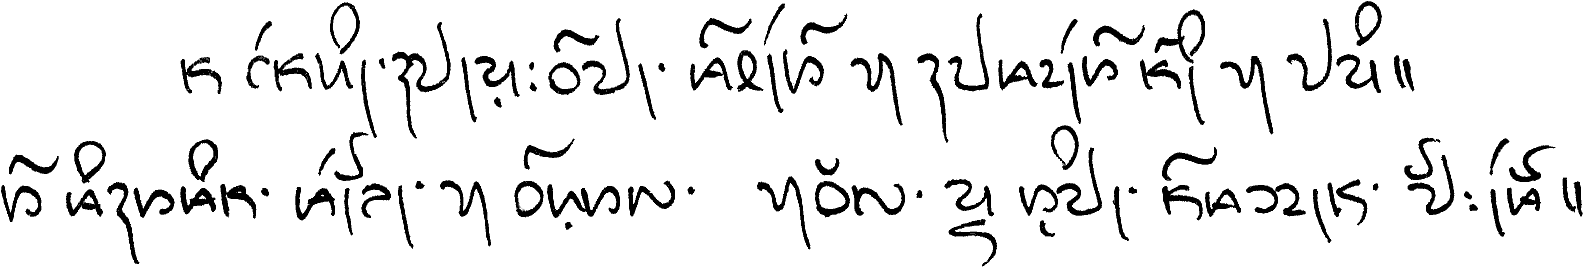
\includegraphics[width=0.75\linewidth]{images/tahanohand-300dpi-bw.png}
\label{fig:thhand}
\end{figure}

Many letter shapes become simplified, specifically \ayr{b}~\orth{ba}, 
\ayr{g}~\orth{ga}, \ayr{k}~\orth{ka}, \ayr{n}~\orth{na}, \ayr{N}~\orth{nga}, 
the vowel carrier \ayr{ʔ}, and the vowel \ayr{*i}~\orth{i}. Not shown here is 
the the vowel length diacritic, \ayr{*aa}, which is simplified to a reverse 
\textit{C} shape. The abbreviation \xayr{\&}{nay}{and} is used throughout, 
though in a shape that is more similar to its `angular' form \ayr{\itshape \&}. 
\ayr{n}~\orth{na} is also taken from the `angular' style \ayr{\itshape n}, which 
opens the possibility that this is actually the basic shape rather than the 
`book' style's \ayr{n}, or both are different developments from a shared 
ancestor.

\index{Tahano Hikamu!blackletter style}
Most recently, I also wondered what Tahano Hikamu might look like if they were 
adapted to European blackletter style with its characteristic broken arches. 
This, of course, constitutes a sharp contrast to Ayeri's usual look and feel, 
which made the experiment all the more interesting, though decidedly 
non-`canonic'. \autoref{fig:thblack} shows what our example passage might have 
looked like at a time when Gothic book hands flourished.

\begin{figure}[ht]\centering
\caption{Tahano Hikamu, `blackletter style'}

\includegraphics[width=0.75\linewidth]{images/tahanoblack-300dpi-bw.png}
\label{fig:thblack}
\end{figure}

The letter shapes from the `book' style stay largely intact here, though all 
curves are broken up into at least two strokes, and strokes from the bottom 
left to the top right, which would push a quill in a way that causes ink to 
splatter, are avoided completely. The characters that differ most are 
\ayr{g}~\orth{ga}, \ayr{r}~\orth{ra}, \ayr{N}~\orth{nga}, and the vowel 
carrier \ayr{ʔ}. \ayr{n}~\orth{na} again appears in the `angular' shape, though 
without its descender word-internally and in the abbreviation \rayr{\&}{nay}. 
\ayr{t}~\orth{ta} comes with a horizontal stroke instead of a curl at the 
bottom; \ayr{s}~\orth{sa} gains a descender, as does \ayr{r}~\orth{ra}. Not 
shown here either are changes to the `large' diacritics.

\index{Tahano Hikamu|)}
